\section{Frekvensblandare}
\label{blandare}
\index{blandare}
\index{frekvensblandare}
\index{mixer}

\subsection{Grundprinciper}

En anordning som blandar signaler för att skapa andra kallas som
namnet säger för \emph{blandare} (eng. \emph{mixer}). Blandare används både i mottagare och
sändare och funktionsprinciperna är lika i båda fallen. Vad som
skiljer i stort är hur de används.

Det finns många blandarkopplingar varav de vanligaste beskrivs
här. Enkla typer med vissa nackdelar ställs mot sådana som är mer
komplicerade, men har fördelar.

\begin{figure}
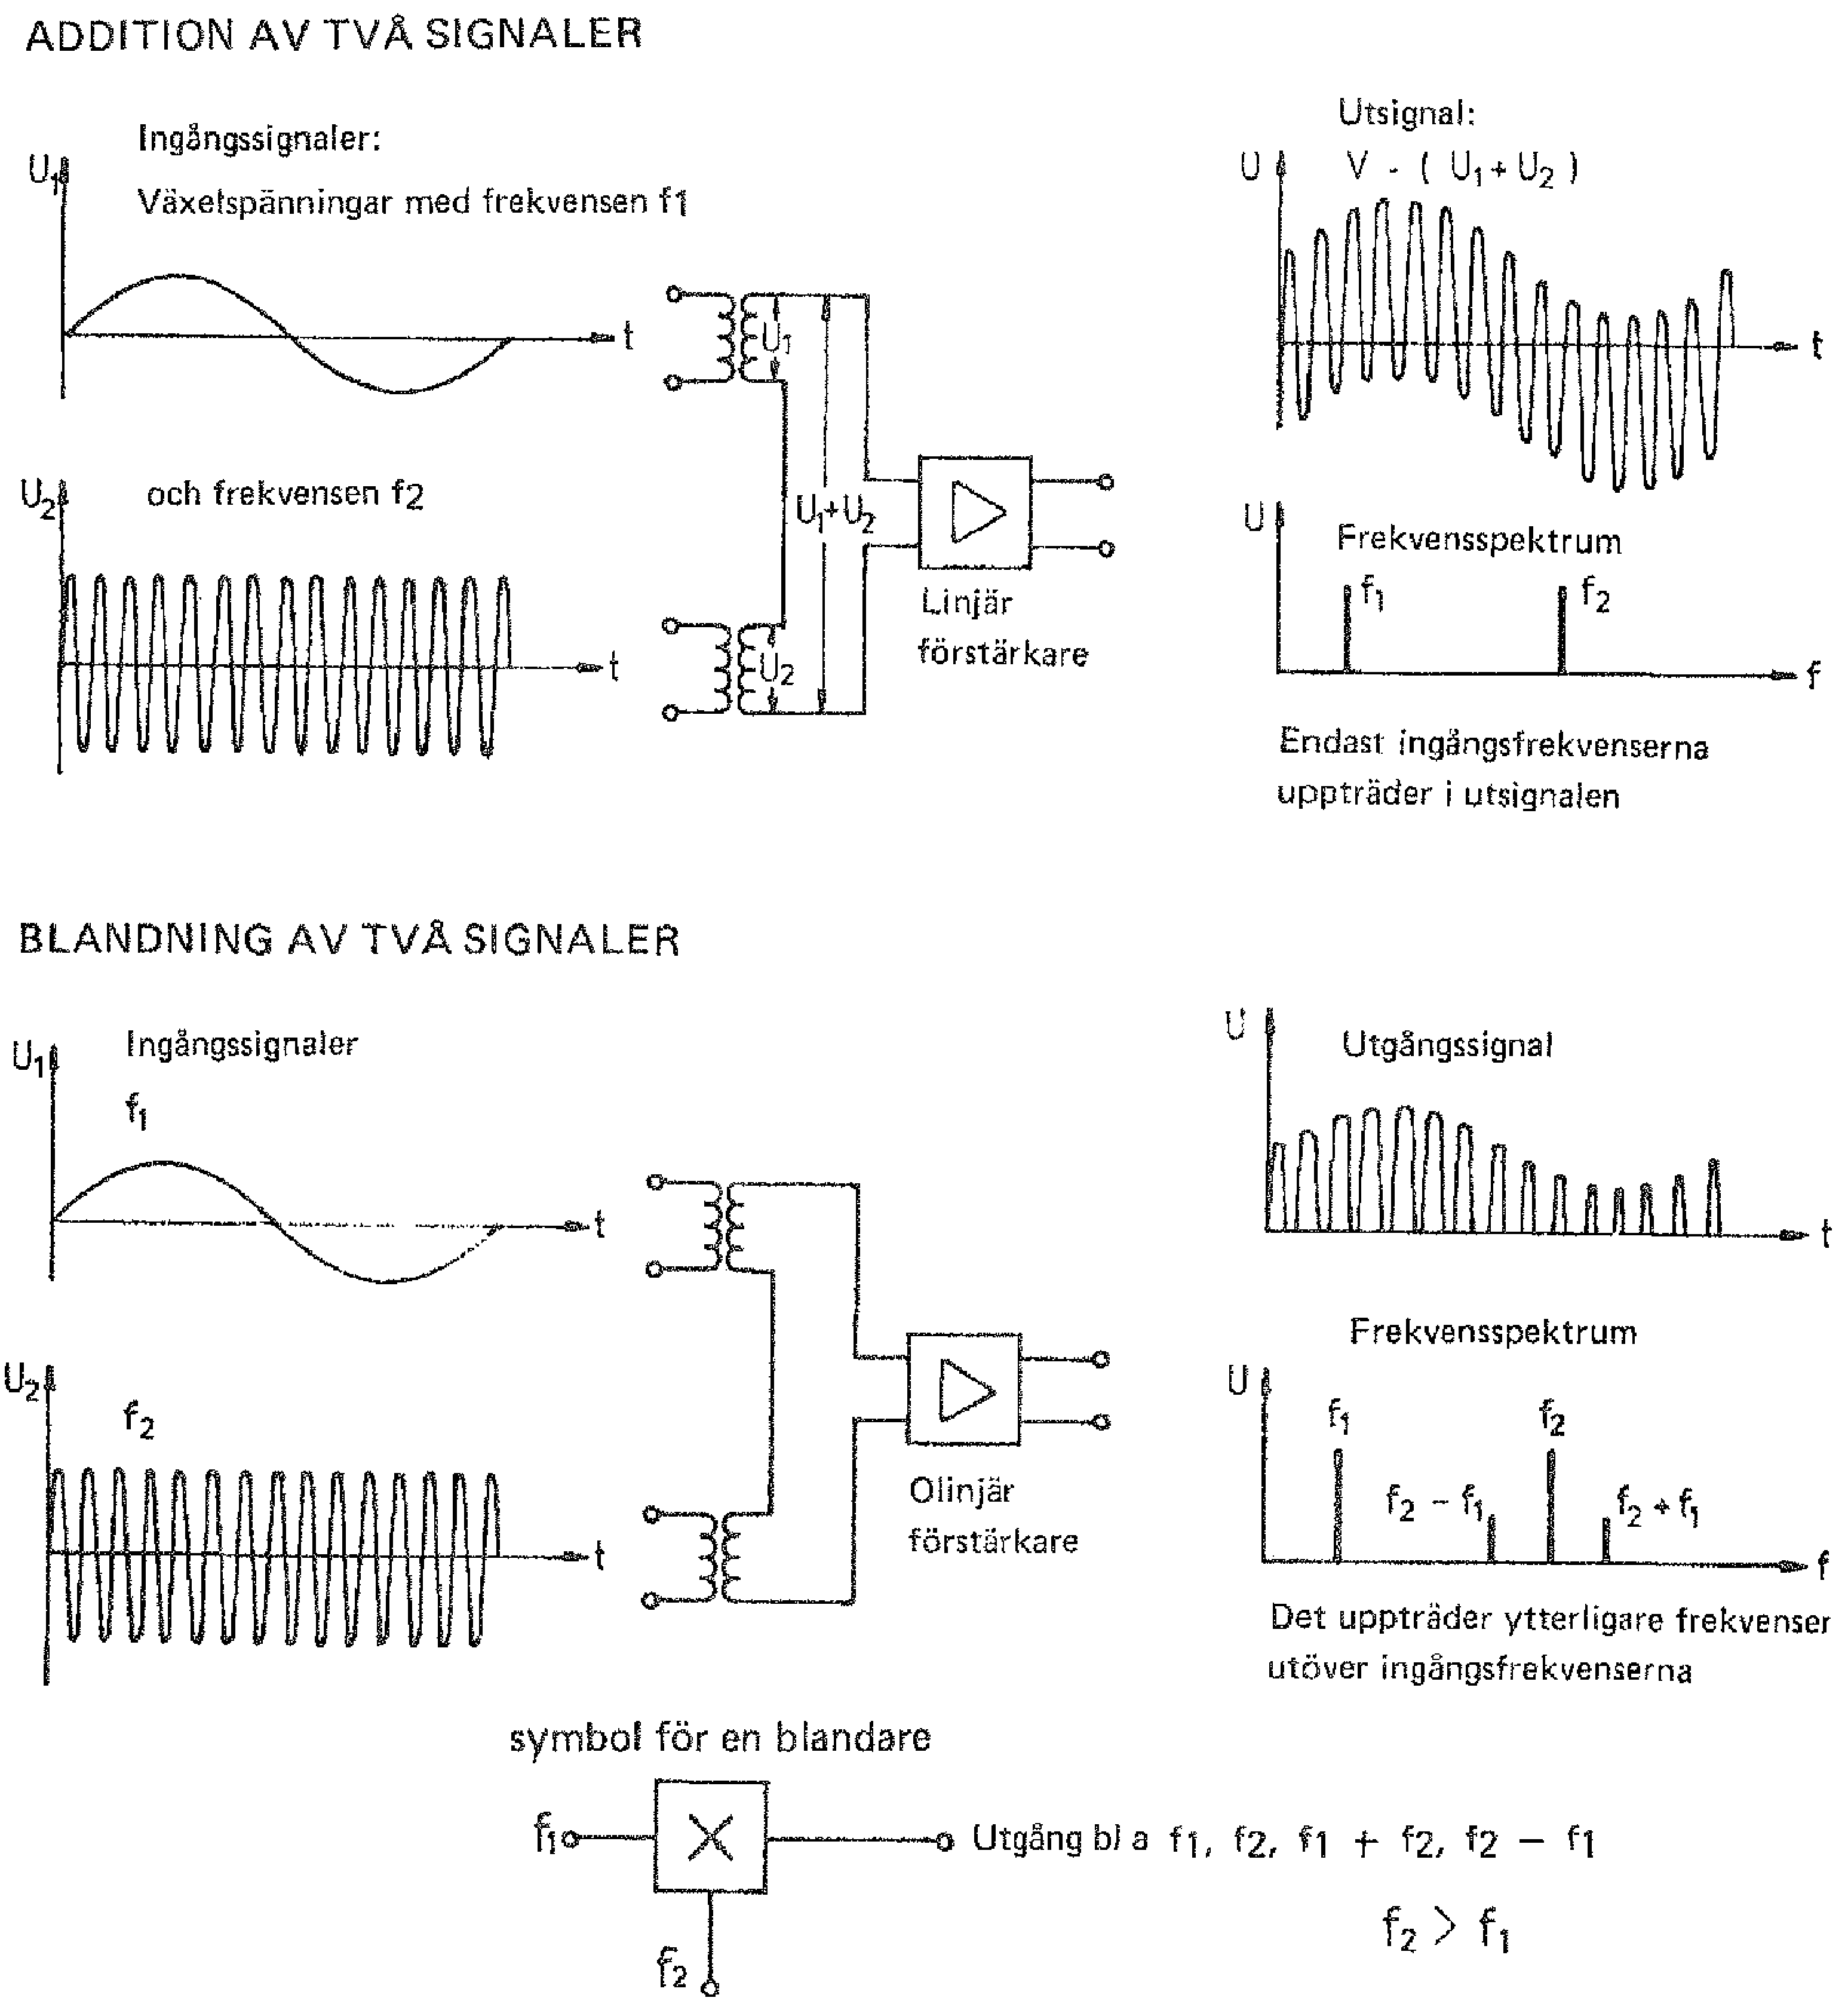
\includegraphics[width=\textwidth]{images/cropped_pdfs/bild_2_3-83.pdf}
\caption{Principer för frekvensblandning}
\label{fig:BildII3-83}
\end{figure}

Bild \ref{fig:BildII3-83}

När en linjär förstärkare matas med två signaler så sammanlagras
de. Den resulterande signalen vid varje tidpunkt är den förstärkta
summan av de inmatade signalerna.

När en olinjär förstärkare matas med två signaler så blandas de med
varandra. Förutom ingångssignalerna uppträder genom blandningen
ytterligare signaler på förstärkarutgången, så kallade
blandningsprodukter.

Två av blandningsprodukterna är särskilt intressanta, det är summan
och skillnaden av ingångssignalernas frekvenser. De oönskade, övriga
blandningsprodukterna filtreras bort med en avstämd krets eller ett
bandpassfilter.

\subsection{Entaktsblandaren}
\index{entaktsblandaren}
\index{blandare!entakts}

\begin{figure}
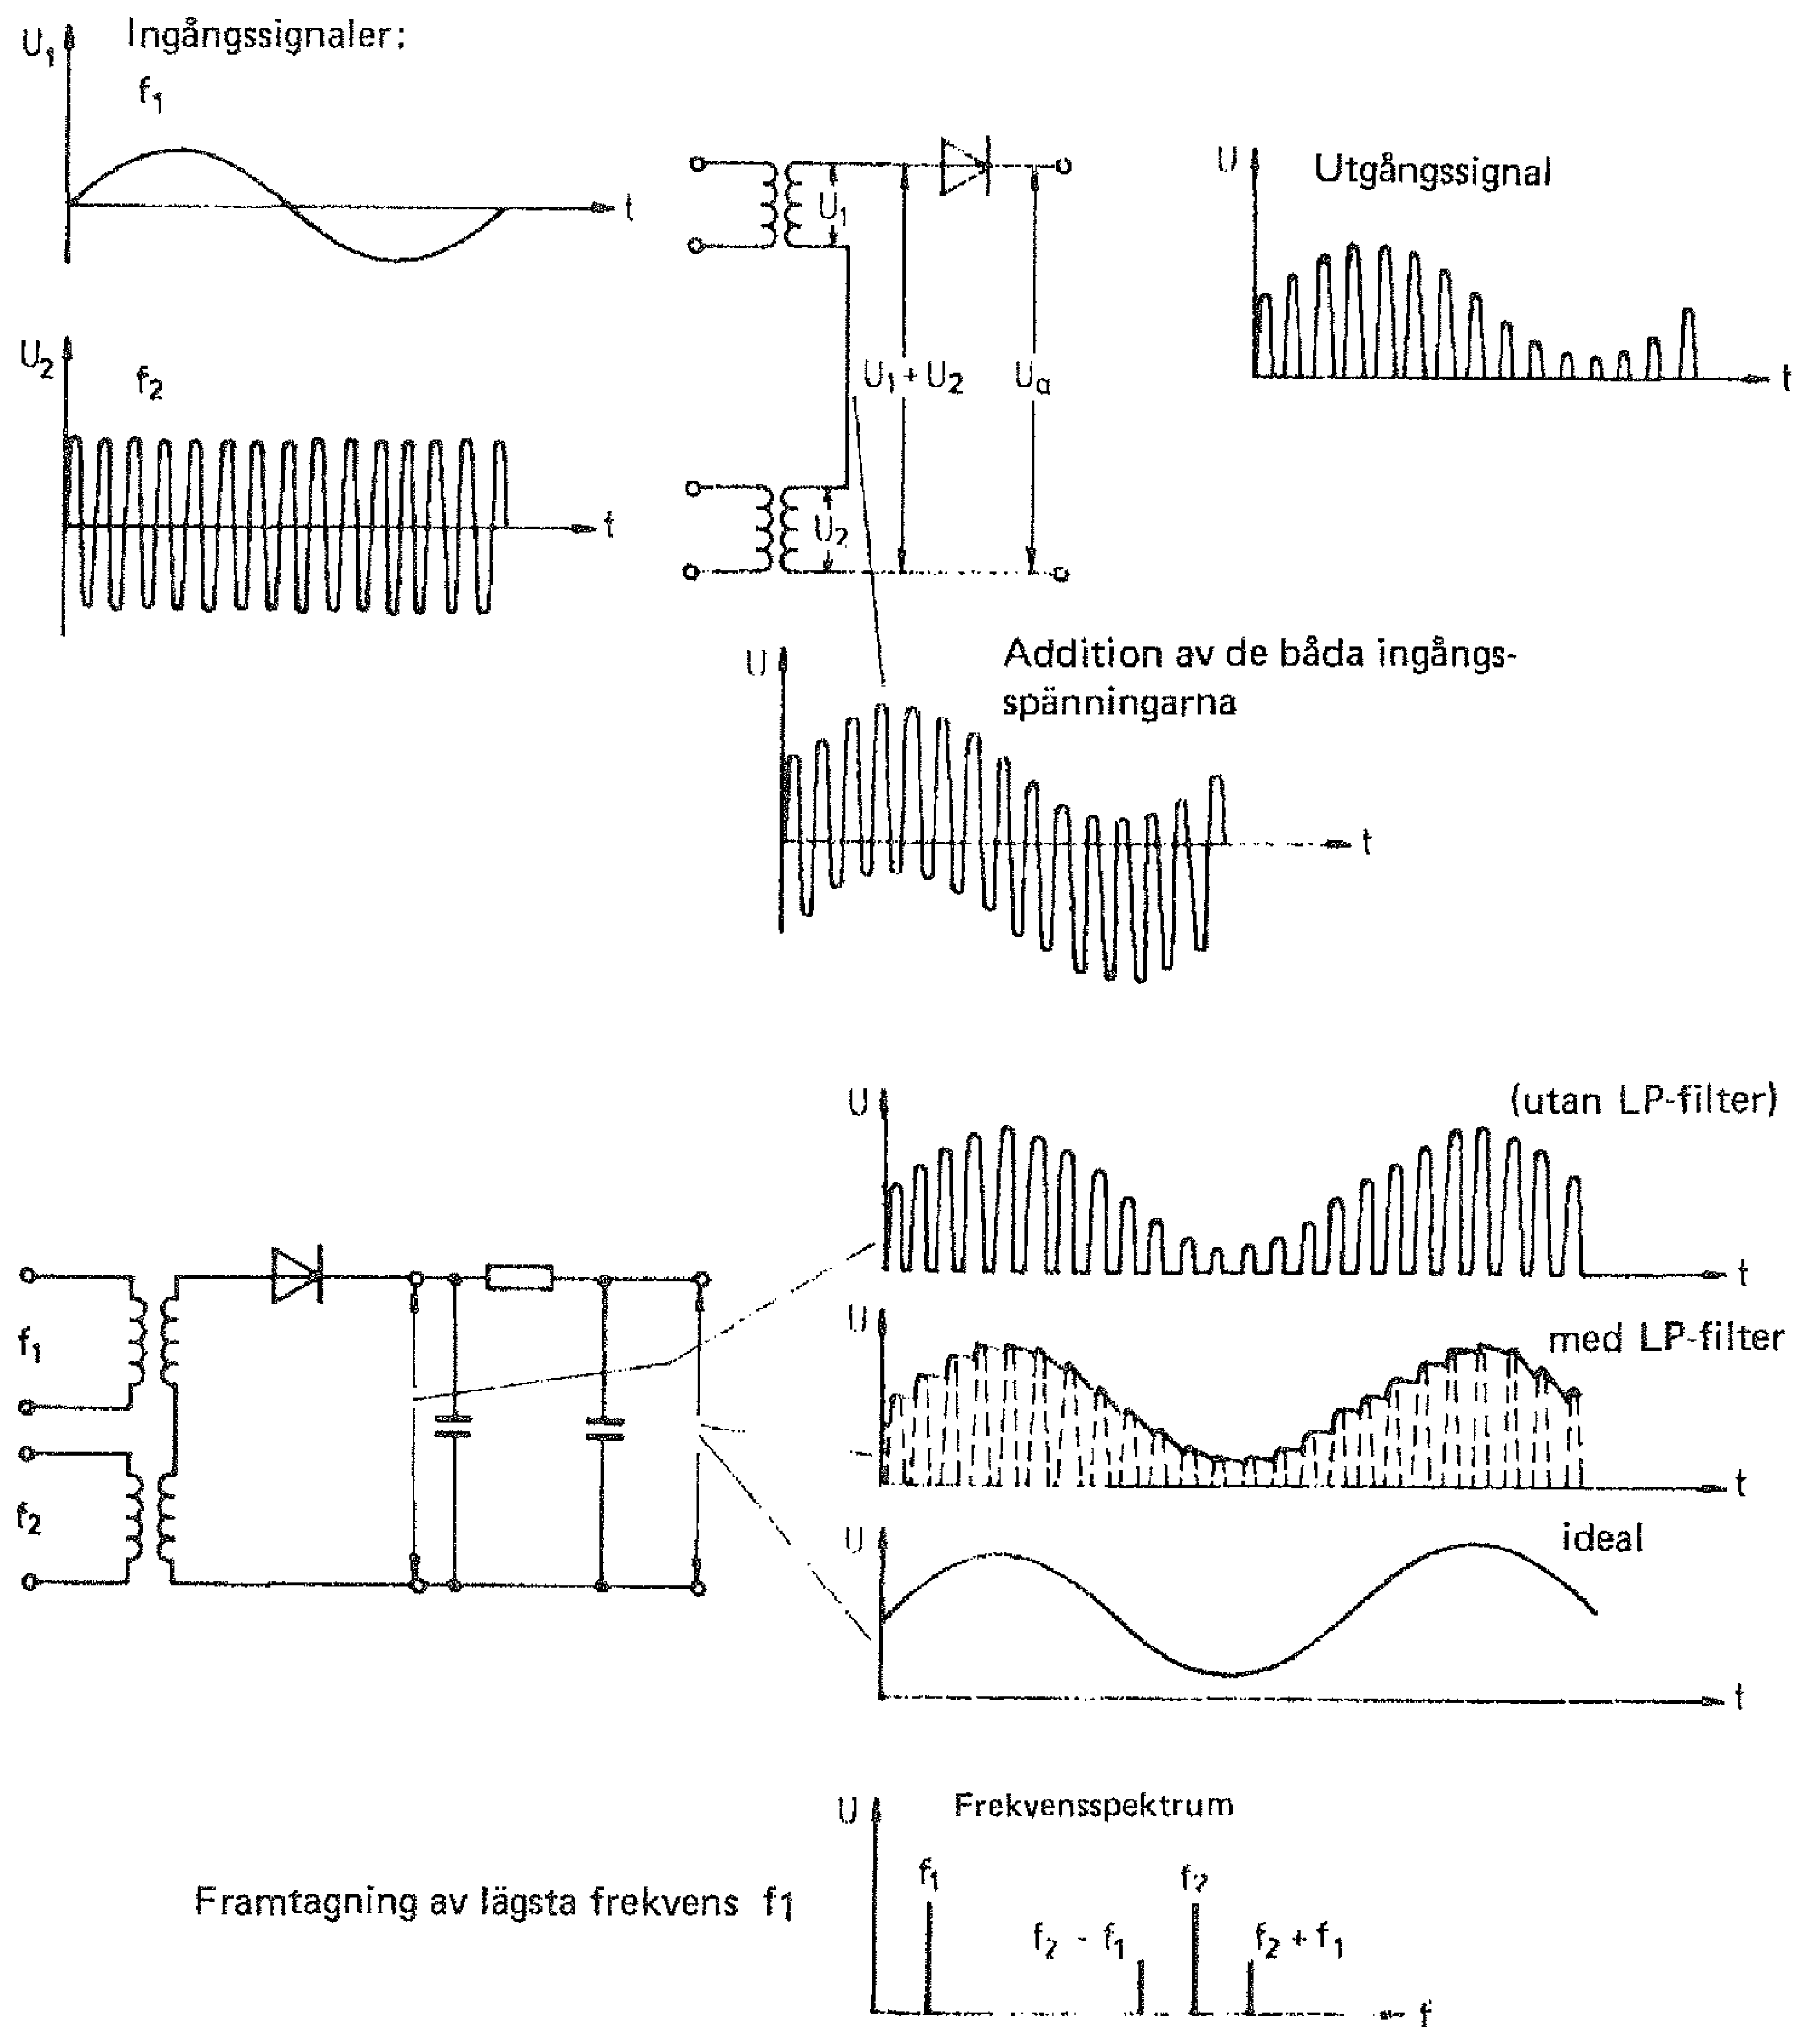
\includegraphics[width=\textwidth]{images/cropped_pdfs/bild_2_3-84a.pdf}
\caption{Entaktsblandaren}
\label{fig:BildII3-84a}
\end{figure}

Bild \ref{fig:BildII3-84a}

Vi kan övertyga oss om, att de fyra blandningsprodukterna verkligen
uppstår. Först undersöker vi den enklaste blandaren, som är ett
olinjärt element i form av en diod.

Det finns ingen förstärkare i kopplingen.
Signalspänningarna adderas genom att de två transformatorernas
sekundärlindningar är seriekopplade.
Dioden ''förvränger'' kraftigt summaspänningens kurvform.
Beroende av hur dioden är polariserad (vänd i kopplingen) blir den negativa
eller den positiva halvvågen bortskuren.

Signalen på blandarens utgång, alltså efter dioden, innehåller
bl.a. frekvenserna \(f_1, f_2, f_2+f_1, f_2-f_1\). Den lägsta
frekvensen \(f_1\) kan lättast påvisas genom att ansluta ett
lågpassfilter till blandarens utgång.

Resultatet kan studeras med ett oscilloskop. Liksom på bilden ser man
då att kondensatorn laddas upp till den positiva halvvågens toppvärde
och med gott närmevärde följer kurvformen på \(f_1\).

\begin{figure}
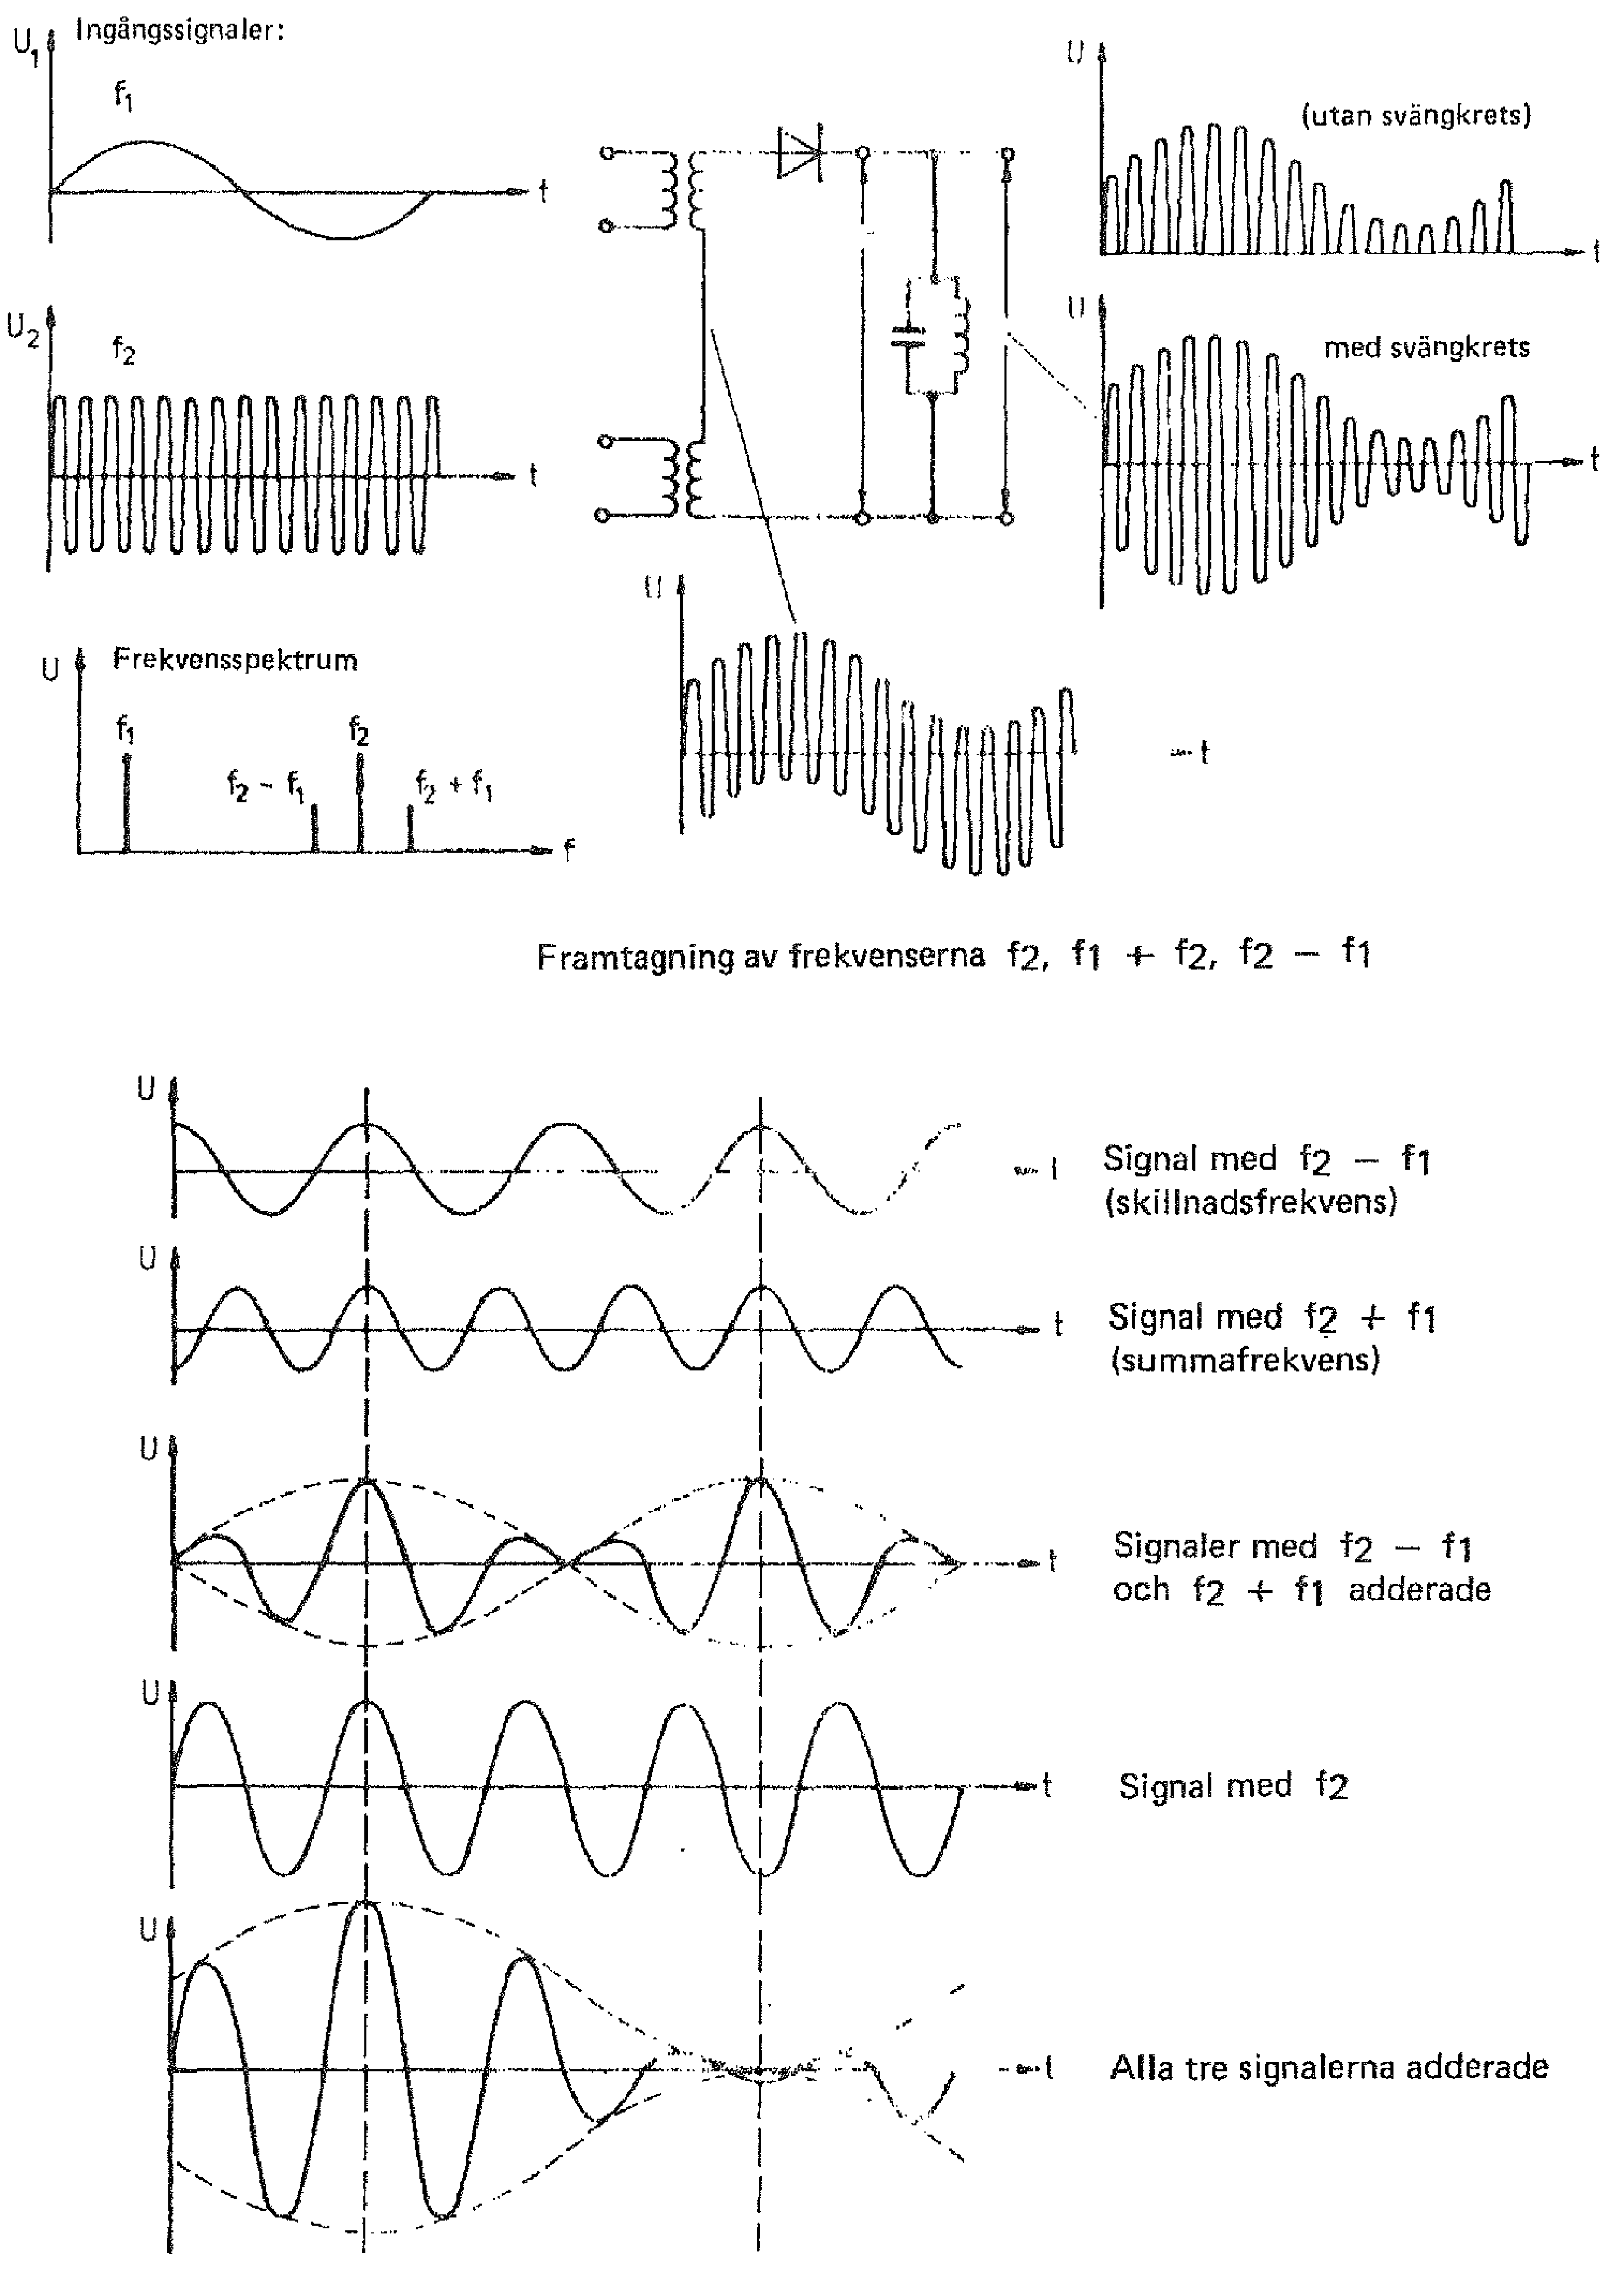
\includegraphics[width=\textwidth]{images/cropped_pdfs/bild_2_3-84b.pdf}
\caption{Entaktsblandaren}
\label{fig:BildII3-84b}
\end{figure}

Bild \ref{fig:BildII3-84b}

En svängningskrets med lämplig bandbredd, och som är avstämd till
resonans frekvensen \(f_2\), ansluts nu till blandarens gång. En
signal med frekvensen \(f_2\) kan då urskiljas och studeras i
oscilloskopet. Svängningskretsen tillförs energi under de positiva
halvvågorna. Energin i svängningskretsen kompletterar med den negativa
halvvågen, varvid en del av kretsens energi förbrukas.  Därför har de
positiva och negativa halvvågorna inte samma amplitud (toppvärde).

Det syns i oscilloskopet hur amplituden ''svävar''. Av detta dras
slutsatsen att signalen består av fler frekvenser än \(f_2\). Signalen
är sammansatt av \(f_2, f_2+f_1\) och \(f_2-f_1\). Signalen \(f_1\)
ligger utanför svängningskretsens selektiva område och är därför
bortfiltrerad (undertryckt). Blandningsprodukterna \(f_2 + f_1\) och
\(f_2 - f_1\) har båda en mindre amplitud än \(f_2\).

Att det finns olika grundtoner och blandningsprodukter kan bevisas med
en ännu smalare svängningskrets med variabel frekvensavstämning, se
bildens nedre del.
Vi har hittills utgått från entaktsblandaren.
Mer utvecklade blandartyper, såsom mottaktblandaren och ringblandaren,
producerar färre blandningsprodukter.

\subsubsection{Mottaktsblandaren}
\index{mottaktsblandare}
\index{blandare!mottakts}

\begin{figure}
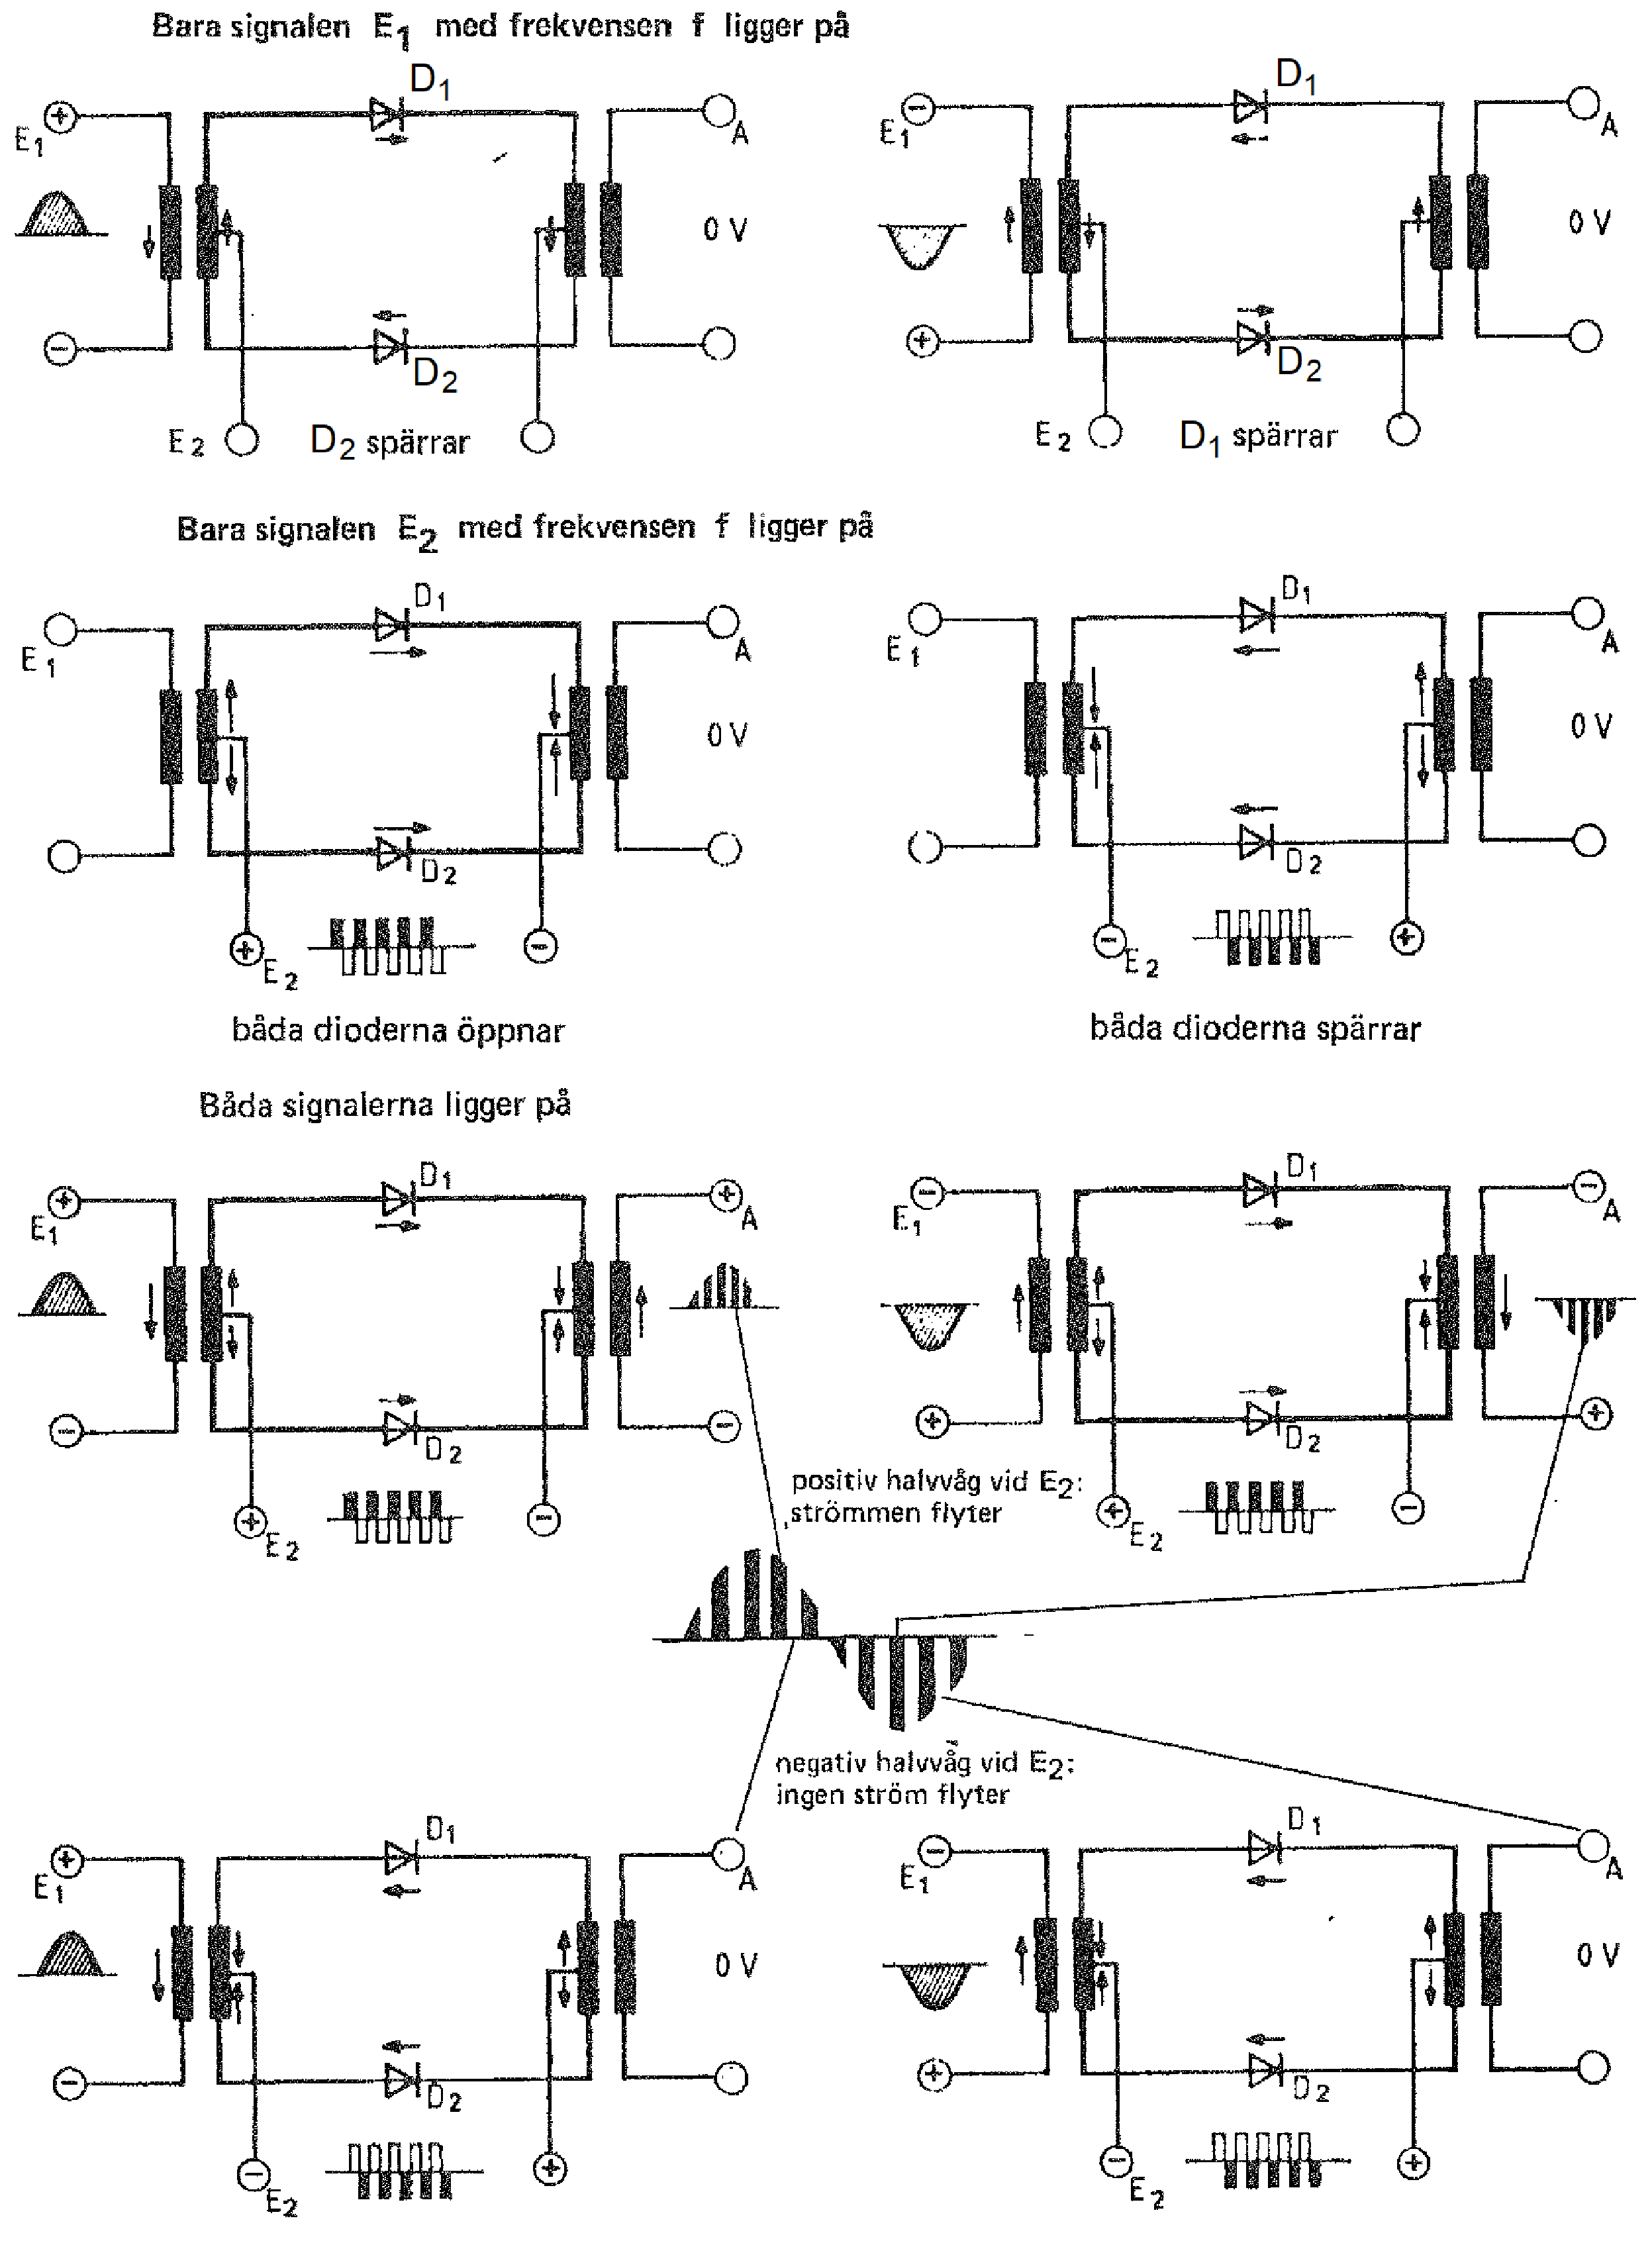
\includegraphics[width=\textwidth]{images/cropped_pdfs/bild_2_3-85.pdf}
\caption{Mottaktsblandaren}
\label{fig:BildII3-85}
\end{figure}

Bild \ref{fig:BildII3-85}

Mottaktblandaren har två dioder, till skillnad mot entaktsblandarens
enda diod. HF-transformatoremas ena lindning har mittuttag.  Ingången
\(E_1\) ligger på den ena transformatorns primärlindning. Ingången
\(E_2\) 1igger över de båda mittuttagen. Utgången ligger på den andra
transformatorns sekundärlindning.

Ingången \(E_1\) matas med en signal med en låg frekvens
\(f\). Eftersom en av de båda dioderna alltid spärrar, så flyter det
ingen ström. De streckade pilarna visar endast i vilken riktning
strömmen kunde flyta, om de spärrande dioderna vore öppna. Men så
länge som ingen signal ligger på ingång \(E_2\), uppträder ingen
signal på utgången.

Signalen på \(E_1\) avlägsnas och i stället matas ingången med en hög
frekvens \(F\). Under den positiva halvvågen är de båda dioderna öppna
och genom båda flyter lika stor ström. De båda transformatorernas
lindningshalvor genomflyts av lika ström i motsatt riktning och då
upphäver magnetfälten i lindningshalvorna varandra och ingen signal
uppträder på utgången.

När signaler läggs båda ingångarna händer följande:

Dioderna öppnar och stänger i takt med signalen på ingång \(E_2\), med
frekvensen \(F\). Den mycket svagare signalen på ingång \(E_1\), med
frekvensen \(f\), kan alltefter polaritet passera diod \(D_1\) eller
\(D_2\). På återvägen överlagras signalen från \(E_1\) på signalen
från \(E_2\). Strömmarna i lindningshalvorna är olika stora. Då
uppträder en signal på utgången.  Efter blandaren följer ett filter
som endast släpper igenom de önskade blandningsprodukterna \(F + f\)
eller \(F - f\).

\subsubsection{Ringblandaren}
\index{ringblandare}
\index{blandare!ring}

\begin{figure}
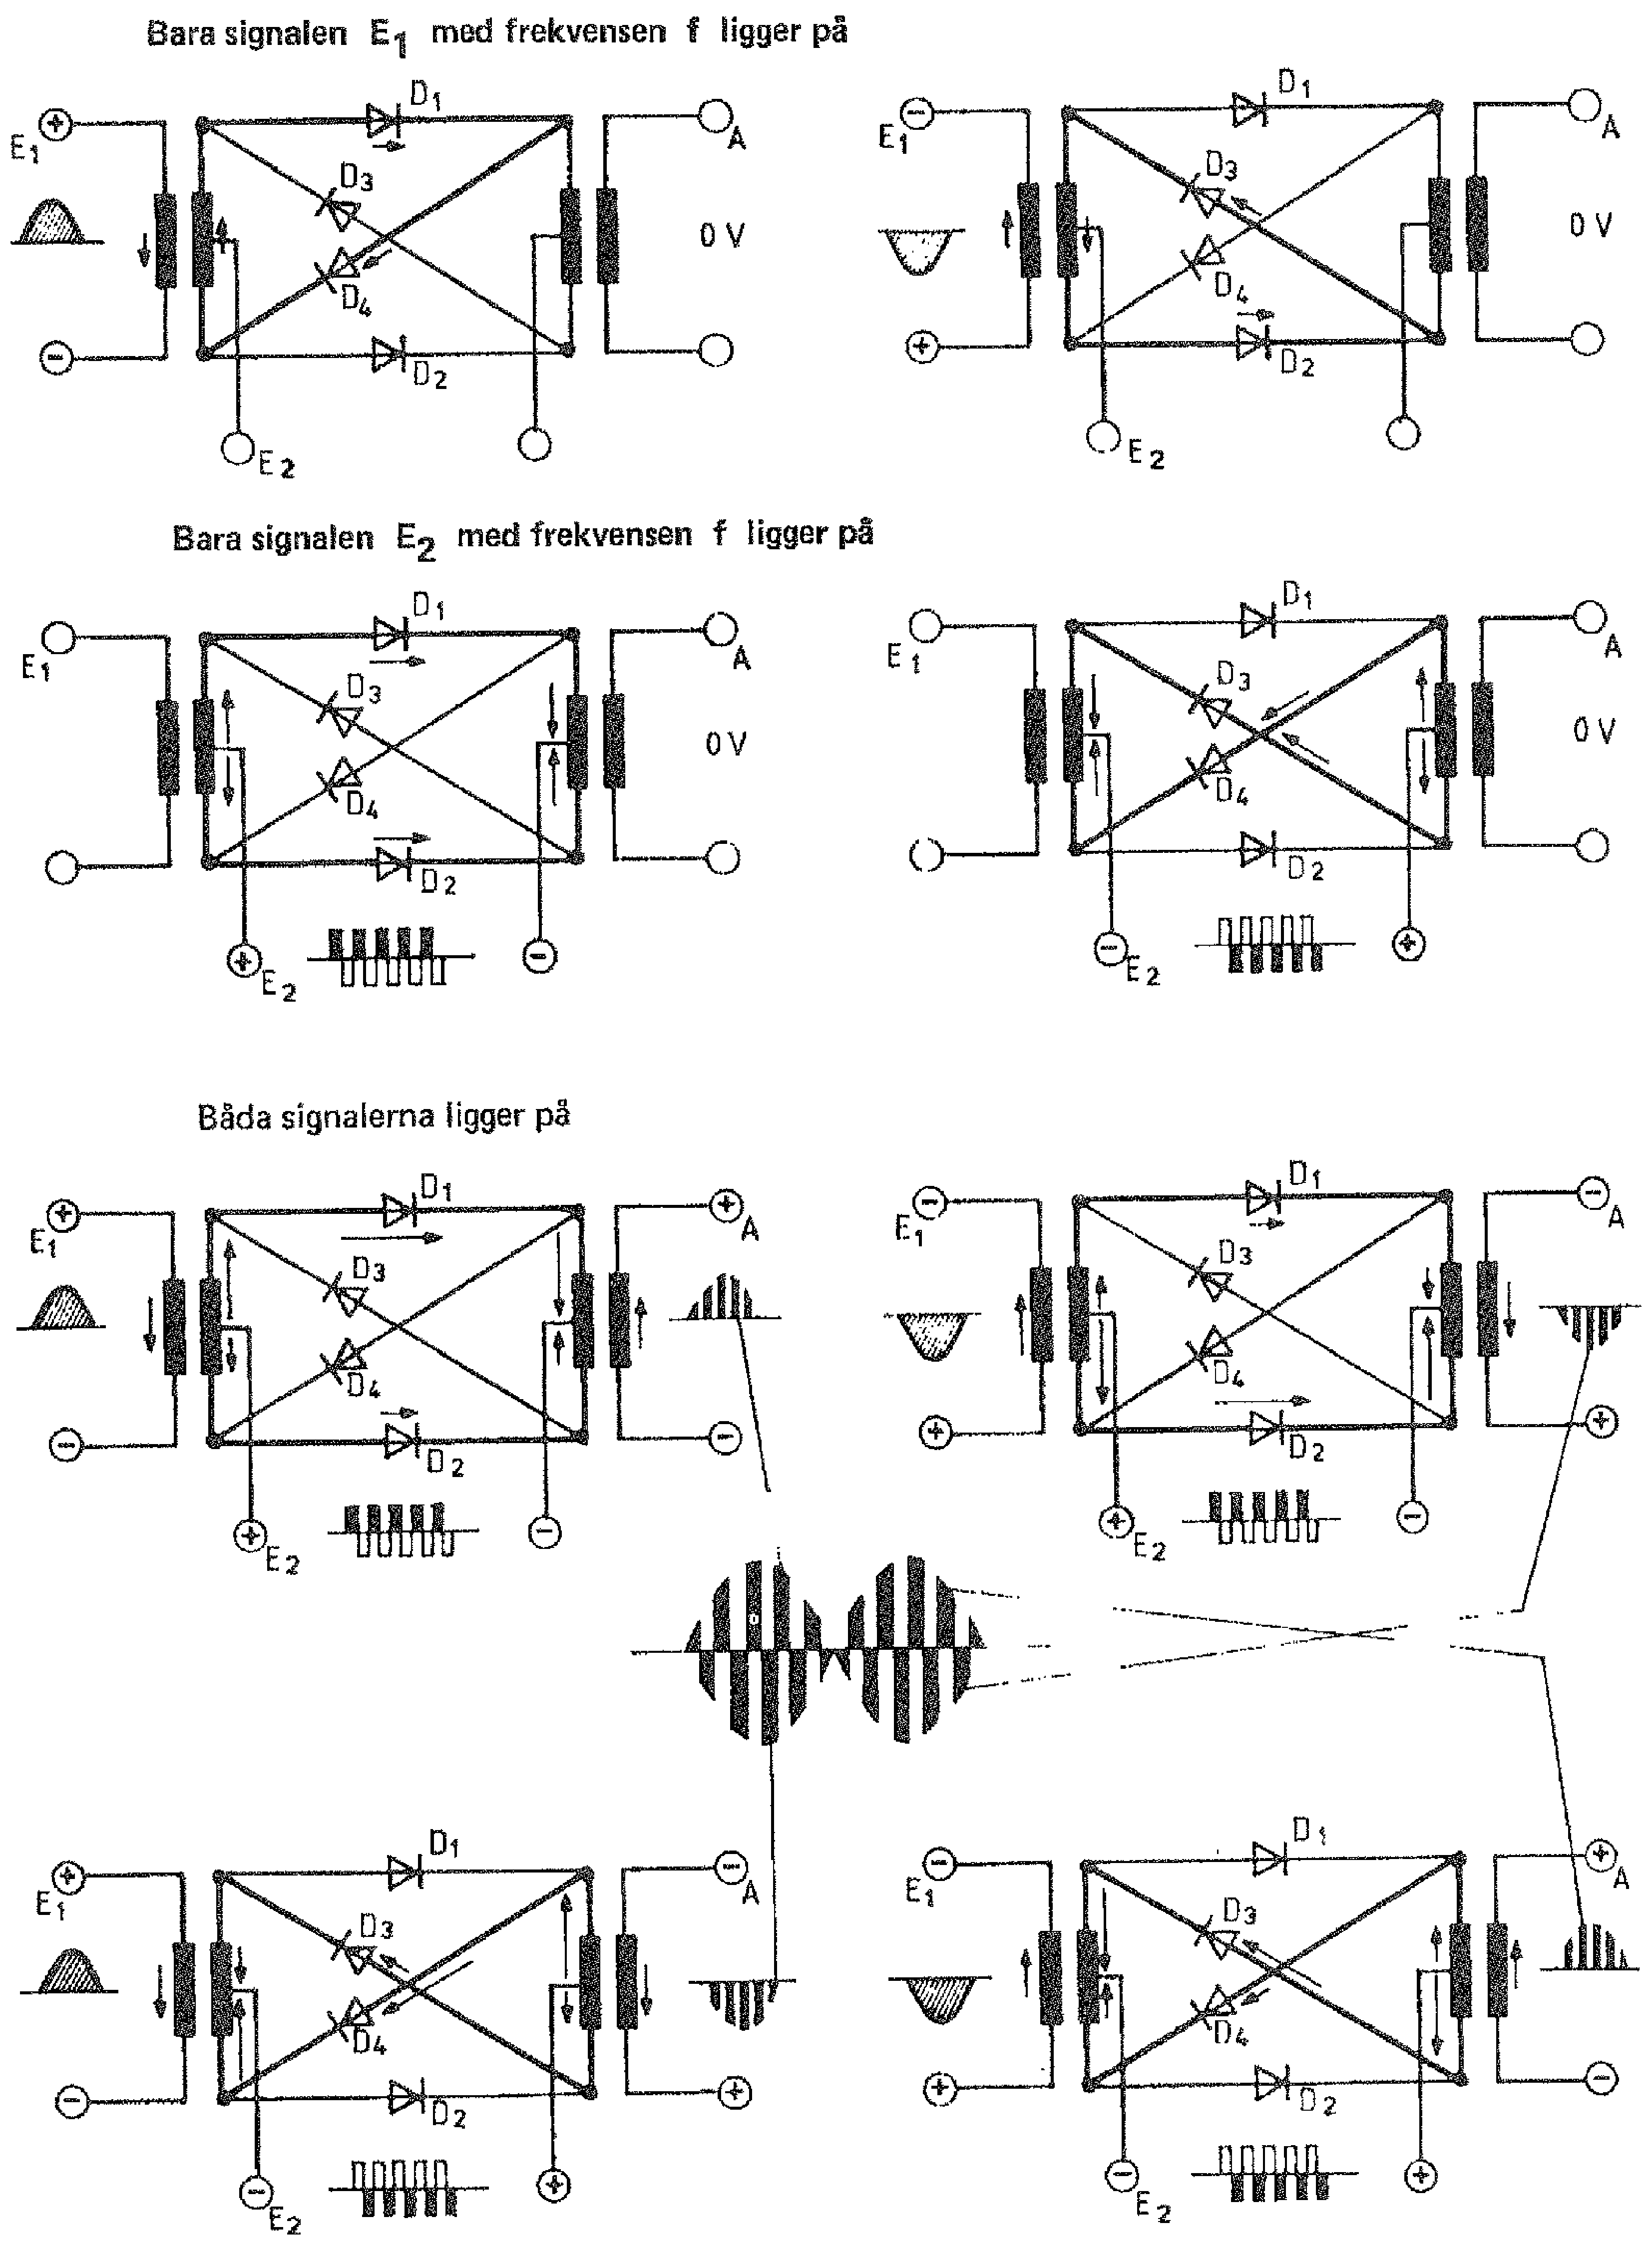
\includegraphics[width=\textwidth]{images/cropped_pdfs/bild_2_3-86.pdf}
\caption{Ringblandaren}
\label{fig:BildII3-86}
\end{figure}

Bild \ref{fig:BildII3-86}

Ringblandaren består av fyra dioder, som är riktade åt samma håll i en
''diodring''. Ingången matas med en signal med en låg frekvens
\(f\). Till skillnad mot i mottaktsblandaren flyter en ström genom
\(D_1\) och \(D_4\) resp. \(D_2\) och \(D_3\), men inte genom
utgångstransformatorn. Ingen signal finns på utgången så länge som
signalen \(F\) saknas.

Signalen på \(E_1\) avlägsnas och i stället matas ingången \(E_2\) med
en hög frekvens \(F\).  Till skillnad mot i mottaktsblandaren flyter
en ström genom dioderna \(D_1\) och \(D_2\) resp. \(D_3\) och \(D_4\)
och då upphäver magnetfälten i transformatorernas lindningshalvor
varandra. Ingen signal finns på utgången, så länge som signalen \(f\)
saknas.

När signaler läggs på båda ingångarna händer följande:

De fyra dioderna kommer att öppna och stänga parvis. Som i
mottaktblandaren överlagras strömmen från ingång \(E_1\) på den ström
som dioderna öppnar för.

Här utnyttjas båda halvperioderna av \(F\). Strömmarna i
lindningshalvorna blir olika stora. På utgången uppträder då en
signal. Efter blandaren följer ett filter som släpper igenom de
önskade blandningsprodukterna.

\subsection{Jämförelse av blandare}

\begin{figure}
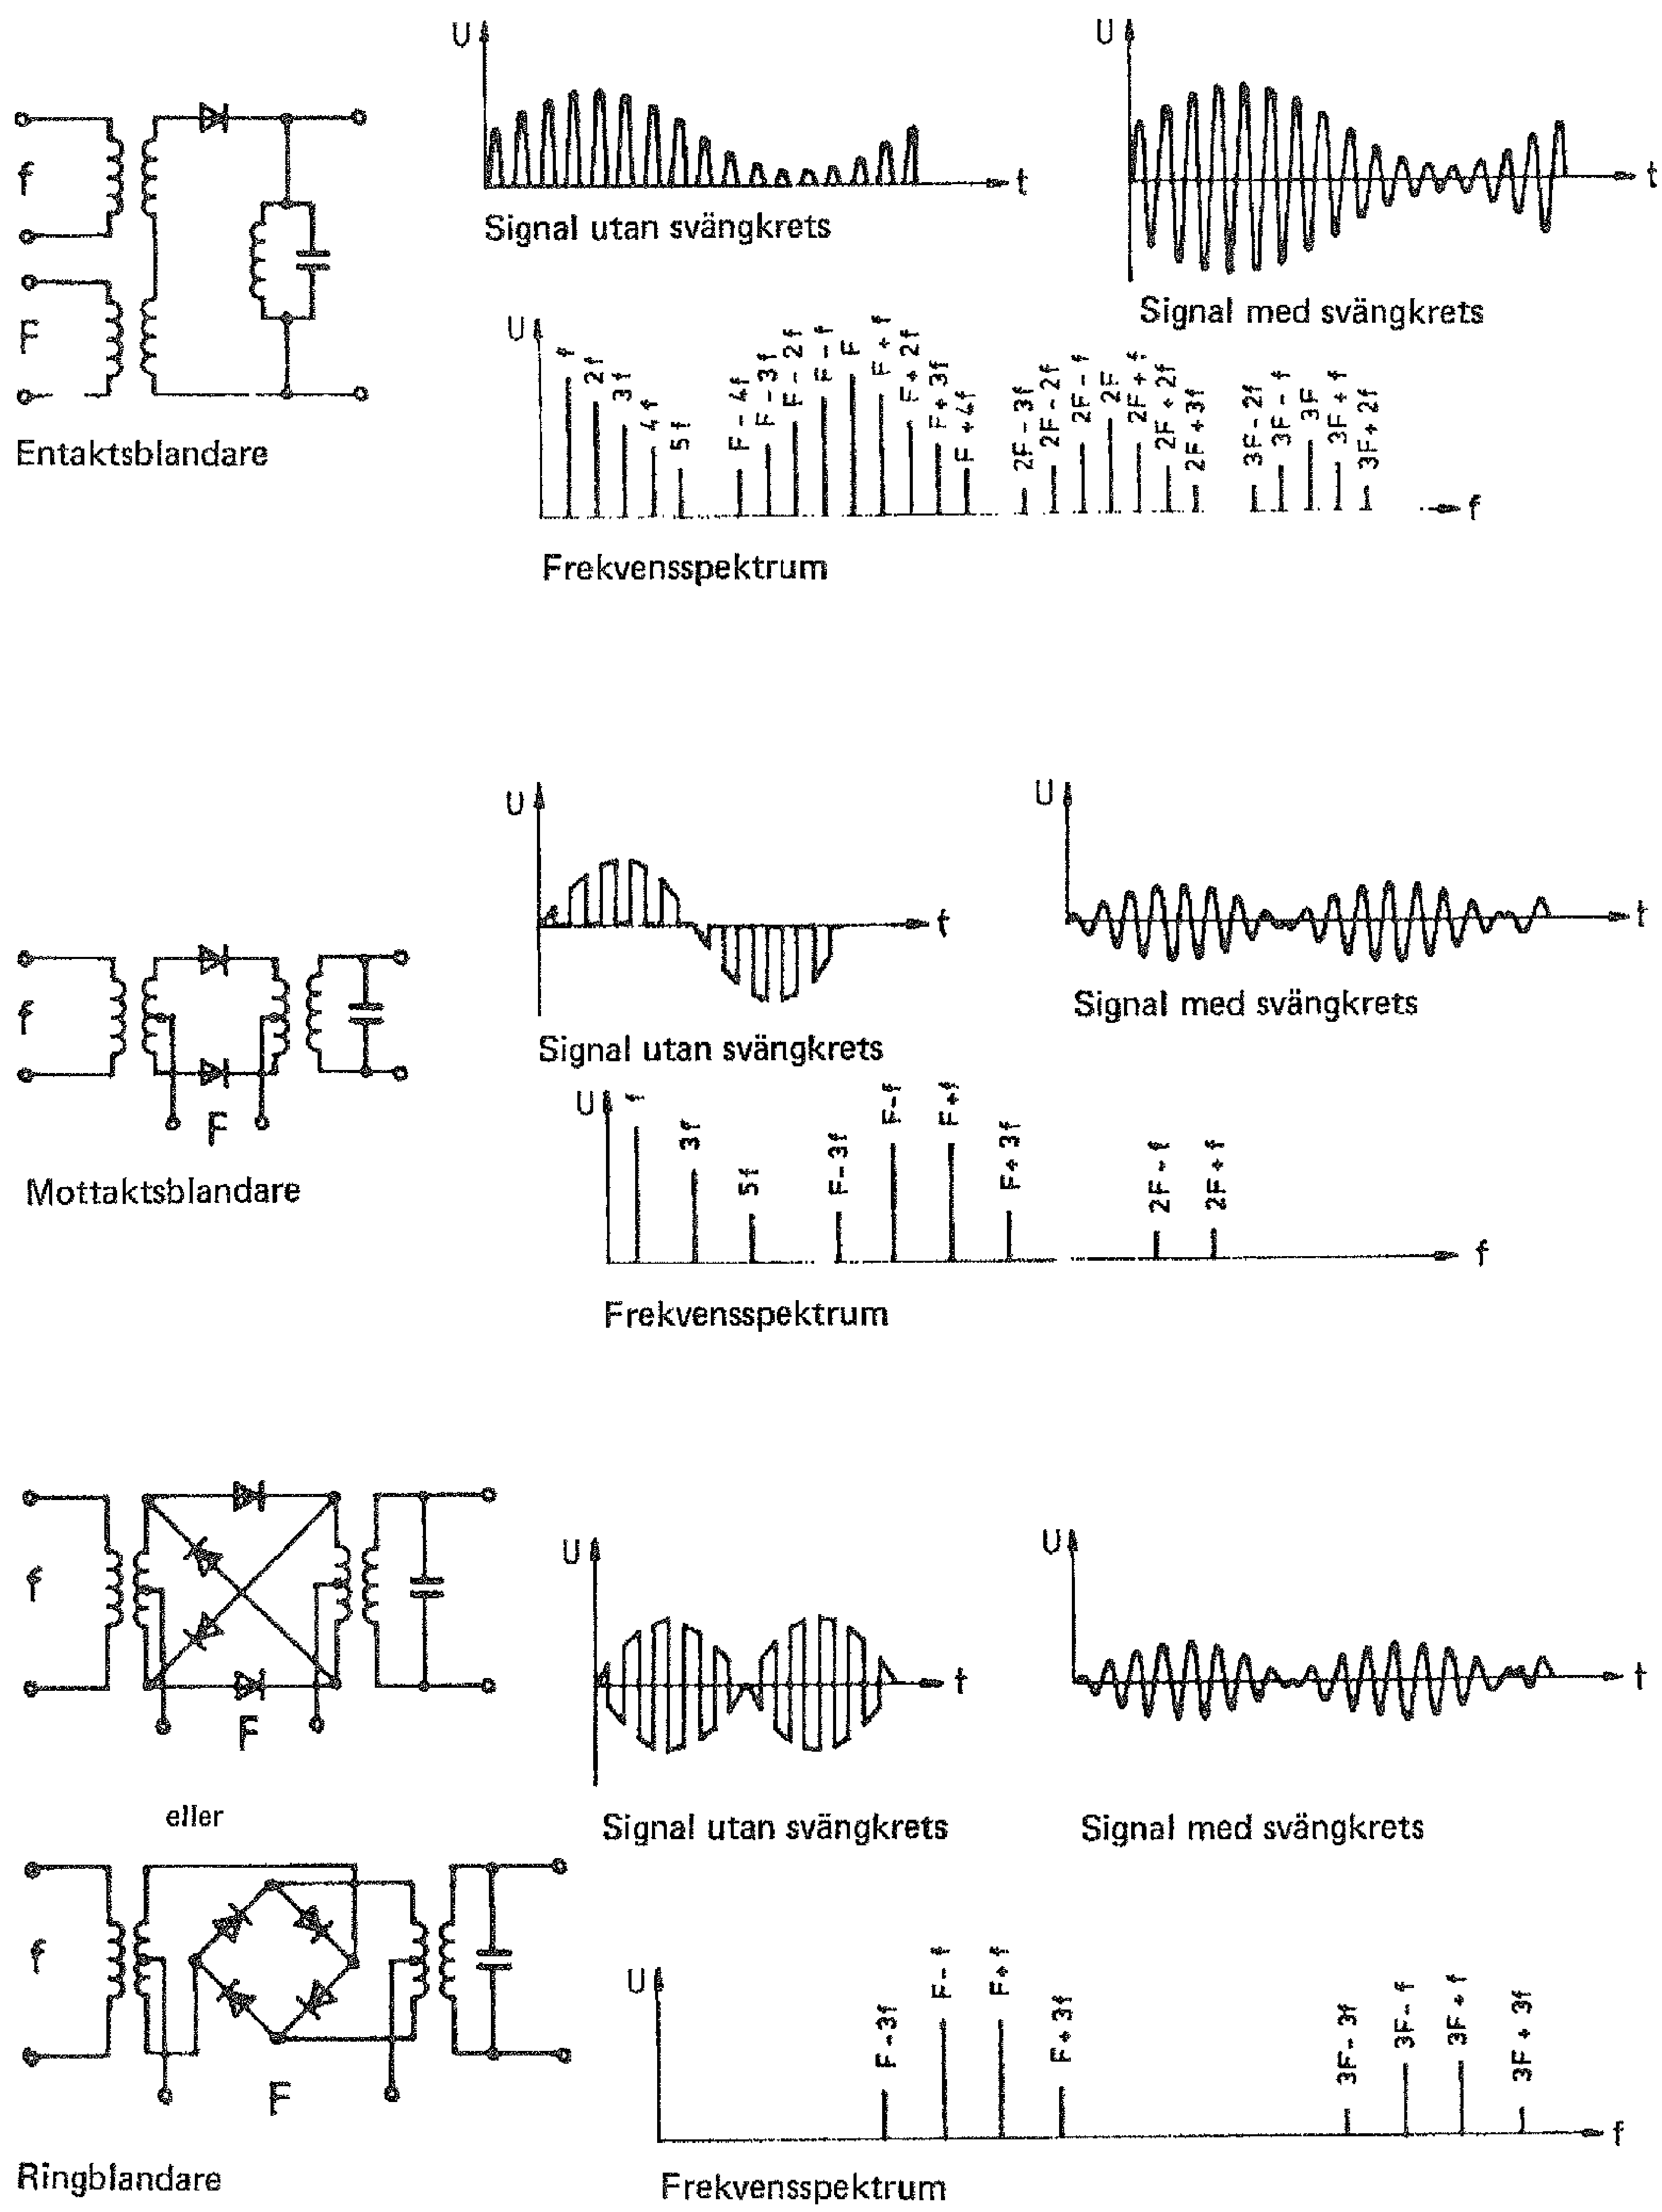
\includegraphics[width=\textwidth]{images/cropped_pdfs/bild_2_3-87.pdf}
\caption{Jämförelse mellan olika blandare}
\label{fig:BildII3-87}
\end{figure}

Bild \ref{fig:BildII3-87}

Bilden visar de tre beskrivna grundkopplingarna och de jämförs med
avseende på frekvensspektrum på utgången.

Vid entaktsblandaren uppträder summafrekvensen \(f + F\) och
skillnadsfrekvensen \(F - f\), vidare ingångsfrekvenserna \(f\) och
\(F\), deras övertoner \(2f\), \(3f\), \(4f\) o.s.v., \(2F\), \(3F\),
\(4F\) o.s.v., liksom deras blandningsprodukter \(F\pm 2f\), \(F\pm
3f\) o.s.v., \(2F \pm f\), \(2F \pm 2f\), \(2F \pm 3f\) o.s.v.

Vid mottaktblandaren saknas frekvensen \(F\) och dess övertoner. Vidare
bortfaller de jämna övertonerna av frekvensen \(f\).

Vid ringblandaren bortfaller ännu fler icke önskvärda signaler,
nämligen ingångssignalerna \(f\) och \(F\) och alla deras övertoner.
Endast blandningsprodukter av udda övertoner uppträder.

På bilden visas det fallet att frekvensen \(f\) är mycket låg och då
ligger blandningsprodukterna mycket nära varandra i frekvens.

Vid entaktsblandaren filtrerar svängningskretsen ut frekvenserna \(F +
f\), \(F - f\), och \(F\). Vid mottakt- och ringblandaren saknas
däremot frekvensen \(F\), den filtrerade signalen innehåller endast
blandningsprodukterna \(F + f\) och \(F - f\). Om dessa båda
blandningsprodukter är väl åtskilda eller svängningskretsen har en
bättre selektionsförmåga, då blir enbart summafrekvensen \(F + f\)
eller skillnadsfrekvensen \(F - f\) framfiltrerad.

Vi har visat tre typer av blandare med passiva komponenter.
Sådana innehåller olinjära dioder (germanium- eller kiseldioder).
Det finns även blandare med aktiva komponenter, d.v.s. elektronrör eller
transistorer (bipolära, FET, MOSFET), men det skulle leda för långt
att gå in på alla olika lösningar.
I kapitlen 4. Mottagare och 5. Sändare beskrivs hur frekvensblandning används
för modulering och demodulering.

\subsection{Icke önskade övertoner och blandningsprodukter}

Varje olinjärt arbetande funktionssteg alstrar förutom nyttofrekvenser
även icke önskade signaler med andra frekvenser. Både önskade och icke
önskade signaler kan bestå av övertoner eller blandningsprodukter
(skillnads- och summatoner) eller bådadera.

Vissa av signalerna filtreras fram för att utgöra nyttosignaler. Andra
signaler filtreras bort, så att t.ex. utsändning inte sker på fel
frekvenser.

\begin{figure}
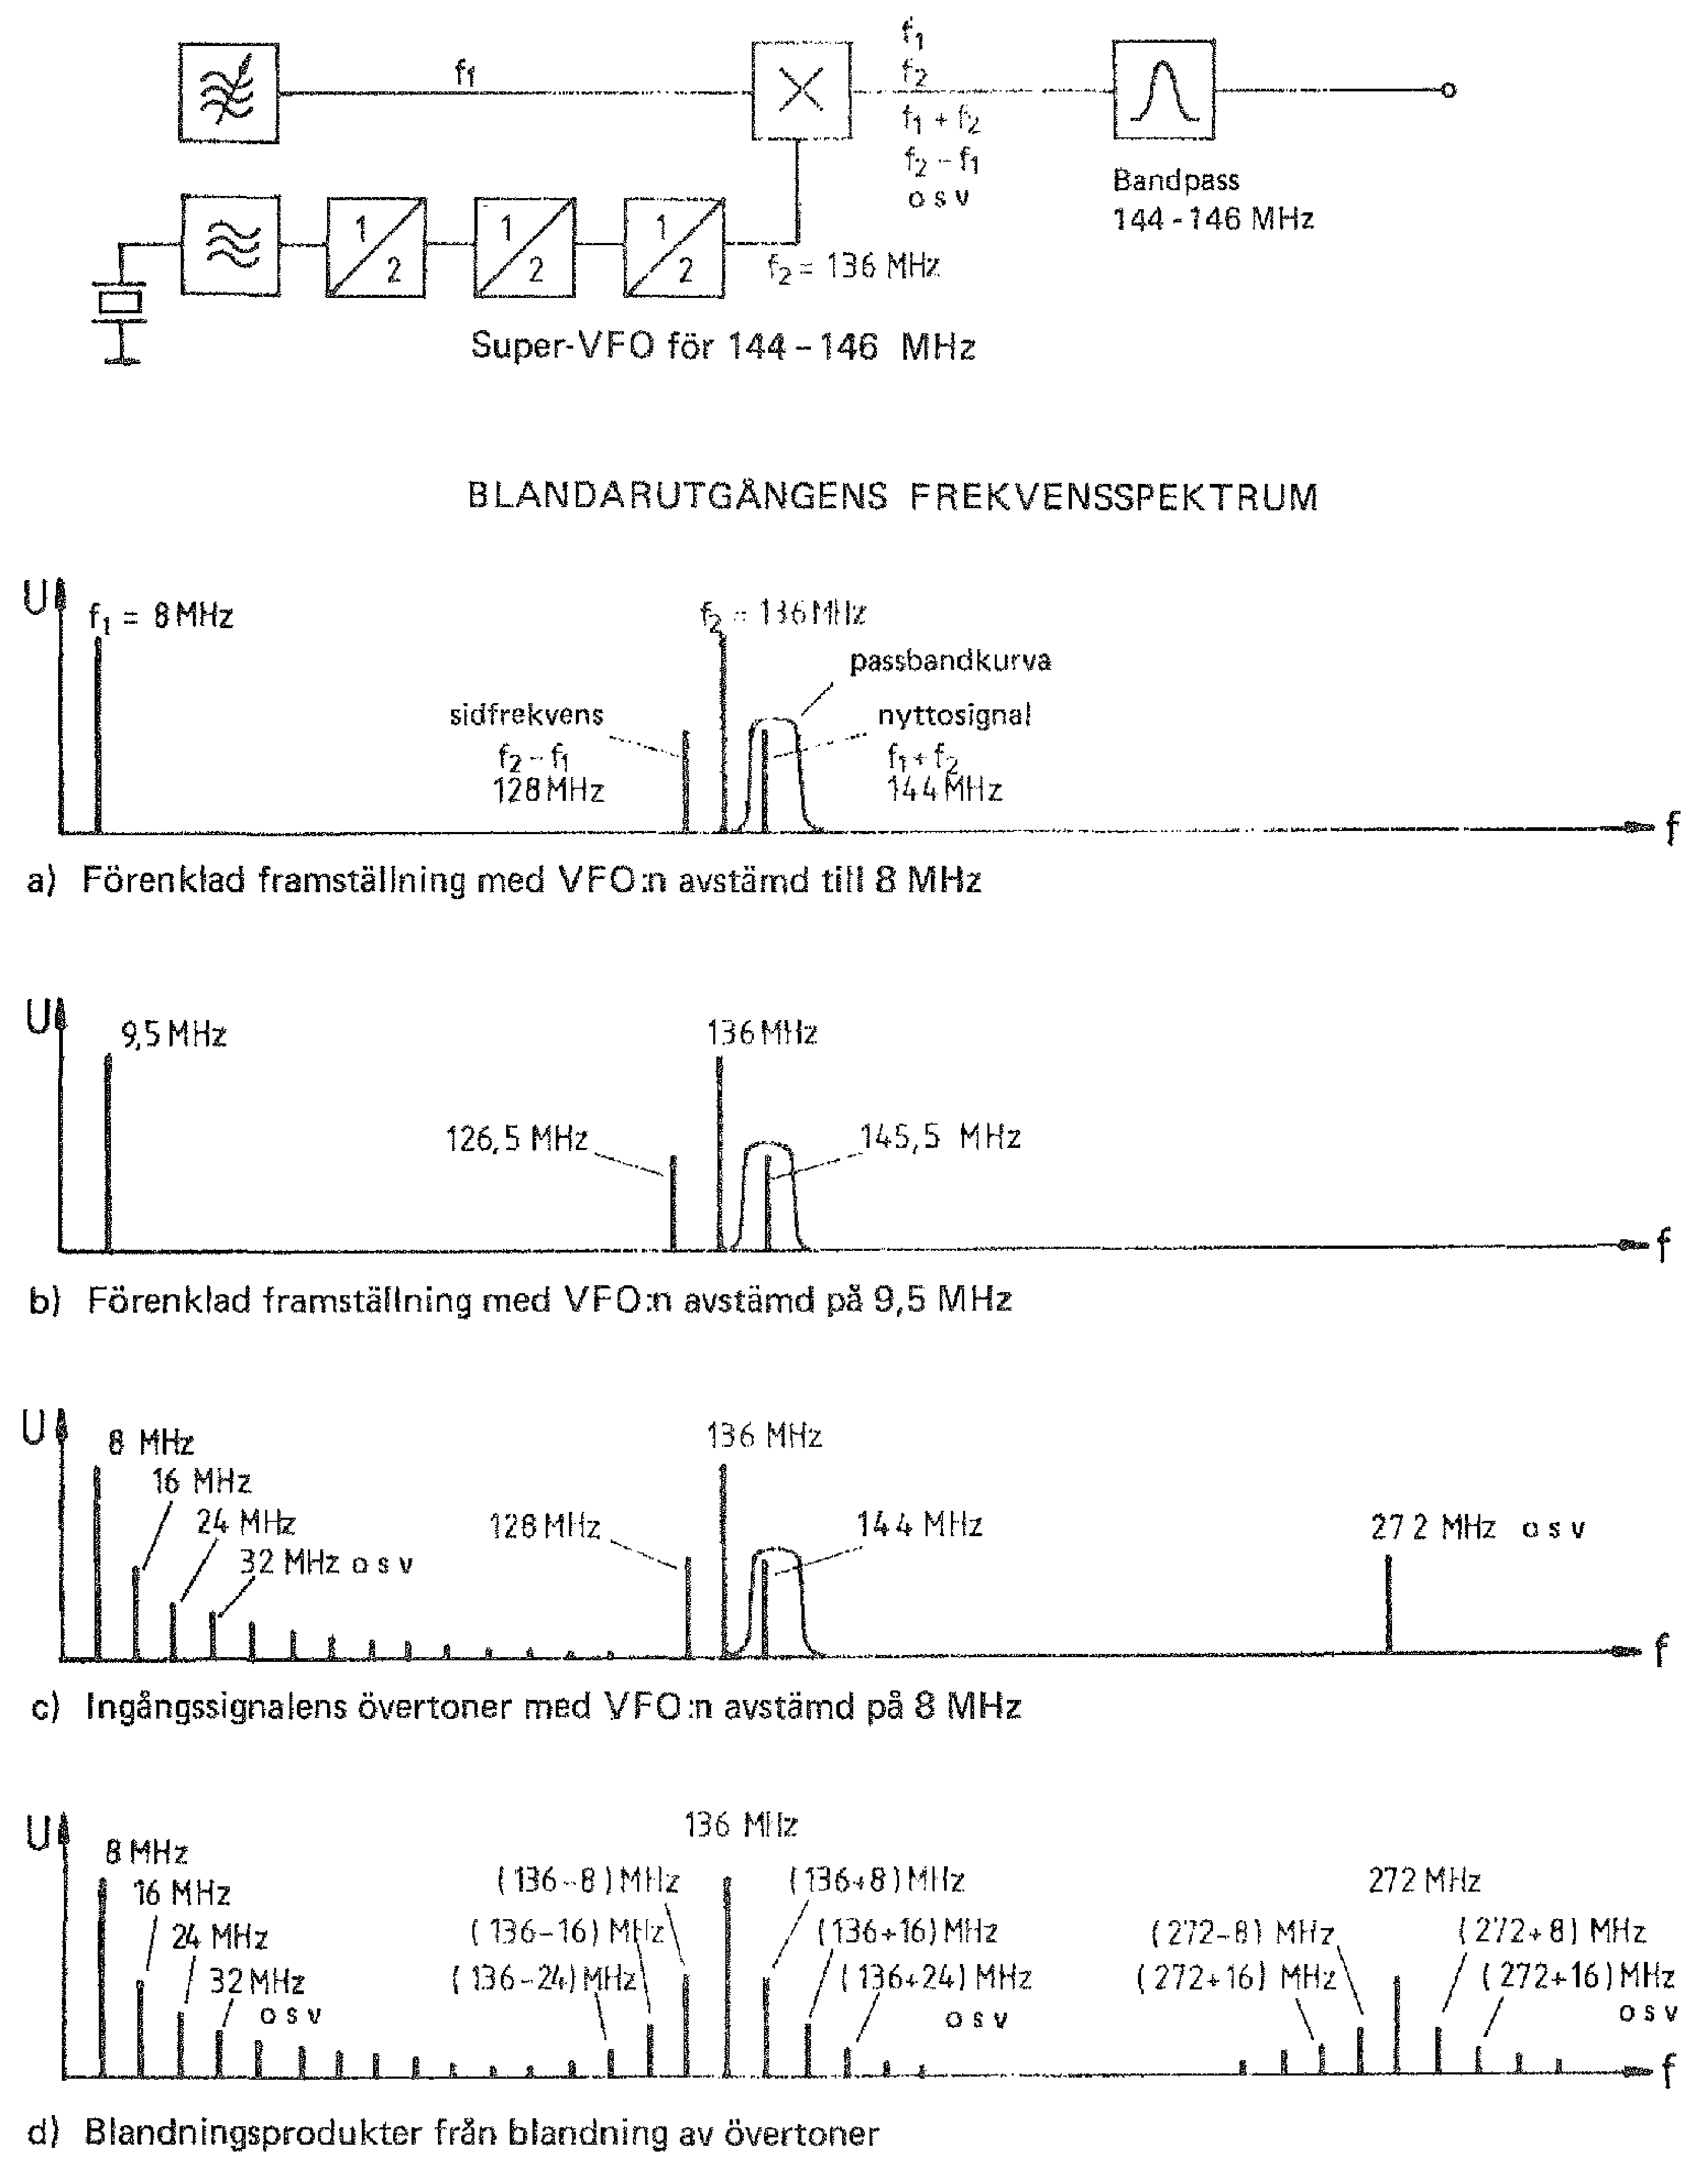
\includegraphics[width=\textwidth]{images/cropped_pdfs/bild_2_3-88.pdf}
\caption{Frekvensspektrum från en Super-VFO}
\label{fig:BildII3-88}
\end{figure}

Bild \ref{fig:BildII3-88}

I ett tidigare avsnitt har vi beskrivit en s.k. super-VFO. Vi ska
nu undersöka vilka blandningsprodukter som uppstår i en sådan. De två
mest uppenbara frekvenserna är blandningsprodukterna (summan) i
området 144--146~MHz och (skillnaden) i området 128--126~MHz.

Ut från blandaren finner vi ingångsfrekvensen 136~MHz och dess
övertoner 272~MHz, 408~MHz o.s.v. såväl som VFO-signalen och dess
övertoner. På bilden är VFO-frekvensen 8~MHz och dess övertoner
inritade, d.v.s. 16~MHz, 24~MHz, 32~MHz o.s.v.

Tyvärr bildar också de båda ingångssignalernas övertoner
blandningsprodukter vilket bilden visar.

Bandpassfiltret släpper igenom nyttofrekvensen, men dämpar alla
övertoner och blandningsprodukter. Detta är enklare ju längre ifrån
nyttosignalen de icke önskade signalerna ligger. I vårt exempel faller
VFO-signalens övertoner inom bandpassfiltrets passband på följande
sätt:

\begin{align*}
  &15 \cdot 9,6   &= 144 \text{MHz} \quad \text{till} \quad 15 \cdot 9,733 &= 146 \text{MHz} \\
  &16 \cdot 9,0   &= 144 \text{MHz} \quad \text{till} \quad 16 \cdot 9,125 &= 146 \text{MHz} \\
  &17 \cdot 8,471 &= 144 \text{MHz} \quad \text{till} \quad 17 \cdot 8,588 &= 146 \text{MHz} \\
  &18 \cdot 8,0   &= 144 \text{MHz} \quad \text{till} \quad 18 \cdot 8,111 &= 146 \text{MHz} \\
\end{align*}

%%

Eftersom det här handlar om 15:e -- 18:e övertonerna, så blir
amplituderna så små, att vi kan bortse från dem.

Det är viktigt med goda filter i signalbehandlande funktionssteg. En
god regel är att på ett tidigt stadium filtrera bort oönskade
övertoner och blandningsprodukter -- helst i varje steg -- så att
onödigt komplexa signaler undviks. Det är också viktigt med
frekvensvalet, så att oönskade blandningsprodukter kommer så långt
bort från nyttofrekvensen som möjligt, liksom att endast mycket höga
övertoner med motsvarande små amplituder faller inom det nyttiga
frekvensområdet.
